% Template for PLoS
% Version 3.3 June 2016
%
% % % % % % % % % % % % % % % % % % % % % %
%
% -- IMPORTANT NOTE
%
% This template contains comments intended 
% to minimize problems and delays during our production 
% process. Please follow the template instructions
% whenever possible.
%
% % % % % % % % % % % % % % % % % % % % % % % 
%
% Once your paper is accepted for publication, 
% PLEASE REMOVE ALL TRACKED CHANGES in this file 
% and leave only the final text of your manuscript. 
% PLOS recommends the use of latexdiff to track changes during review, as this will help to maintain a clean tex file.
% Visit https://www.ctan.org/pkg/latexdiff?lang=en for info or contact us at latex@plos.org.
%
%
% There are no restrictions on package use within the LaTeX files except that 
% no packages listed in the template may be deleted.
%
% Please do not include colors or graphics in the text.
%
% The manuscript LaTeX source should be contained within a single file (do not use \input, \externaldocument, or similar commands).
%
% % % % % % % % % % % % % % % % % % % % % % %
%
% -- FIGURES AND TABLES
%
% Please include tables/figure captions directly after the paragraph where they are first cited in the text.
%
% DO NOT INCLUDE GRAPHICS IN YOUR MANUSCRIPT
% - Figures should be uploaded separately from your manuscript file. 
% - Figures generated using LaTeX should be extracted and removed from the PDF before submission. 
% - Figures containing multiple panels/subfigures must be combined into one image file before submission.
% For figure citations, please use "Fig" instead of "Figure".
% See http://journals.plos.org/plosone/s/figures for PLOS figure guidelines.
%
% Tables should be cell-based and may not contain:
% - spacing/line breaks within cells to alter layout or alignment
% - do not nest tabular environments (no tabular environments within tabular environments)
% - no graphics or colored text (cell background color/shading OK)
% See http://journals.plos.org/plosone/s/tables for table guidelines.
%
% For tables that exceed the width of the text column, use the adjustwidth environment as illustrated in the example table in text below.
%
% % % % % % % % % % % % % % % % % % % % % % % %
%
% -- EQUATIONS, MATH SYMBOLS, SUBSCRIPTS, AND SUPERSCRIPTS
%
% IMPORTANT
% Below are a few tips to help format your equations and other special characters according to our specifications. For more tips to help reduce the possibility of formatting errors during conversion, please see our LaTeX guidelines at http://journals.plos.org/plosone/s/latex
%
% For inline equations, please be sure to include all portions of an equation in the math environment.  For example, x$^2$ is incorrect; this should be formatted as $x^2$ (or $\mathrm{x}^2$ if the romanized font is desired).
%
% Do not include text that is not math in the math environment. For example, CO2 should be written as CO\textsubscript{2} instead of CO$_2$.
%
% Please add line breaks to long display equations when possible in order to fit size of the column. 
%
% For inline equations, please do not include punctuation (commas, etc) within the math environment unless this is part of the equation.
%
% When adding superscript or subscripts outside of brackets/braces, please group using {}.  For example, change "[U(D,E,\gamma)]^2" to "{[U(D,E,\gamma)]}^2". 
%
% Do not use \cal for caligraphic font.  Instead, use \mathcal{}
%
% % % % % % % % % % % % % % % % % % % % % % % % 
%
% Please contact latex@plos.org with any questions.
%
% % % % % % % % % % % % % % % % % % % % % % % %

\documentclass[10pt,letterpaper]{article}
\usepackage[top=0.85in,left=2.75in,footskip=0.75in]{geometry}

% amsmath and amssymb packages, useful for mathematical formulas and symbols
\usepackage{amsmath,amssymb}

% Use adjustwidth environment to exceed column width (see example table in text)
\usepackage{changepage}

% Use Unicode characters when possible
\usepackage[utf8x]{inputenc}

% textcomp package and marvosym package for additional characters
\usepackage{textcomp,marvosym}

% cite package, to clean up citations in the main text. Do not remove.
\usepackage{cite}

% Use nameref to cite supporting information files (see Supporting Information section for more info)
\usepackage{nameref,hyperref}

% line numbers
\usepackage[right]{lineno}

% ligatures disabled
\usepackage{microtype}
\DisableLigatures[f]{encoding = *, family = * }

% color can be used to apply background shading to table cells only
\usepackage[table]{xcolor}

% array package and thick rules for tables
\usepackage{array}

\usepackage{csquotes}

% create "+" rule type for thick vertical lines
\newcolumntype{+}{!{\vrule width 2pt}}

% create \thickcline for thick horizontal lines of variable length
\newlength\savedwidth
\newcommand\thickcline[1]{%
  \noalign{\global\savedwidth\arrayrulewidth\global\arrayrulewidth 2pt}%
  \cline{#1}%
  \noalign{\vskip\arrayrulewidth}%
  \noalign{\global\arrayrulewidth\savedwidth}%
}

% \thickhline command for thick horizontal lines that span the table
\newcommand\thickhline{\noalign{\global\savedwidth\arrayrulewidth\global\arrayrulewidth 2pt}%
\hline
\noalign{\global\arrayrulewidth\savedwidth}}


% Remove comment for double spacing
%\usepackage{setspace} 
%\doublespacing

% Text layout
\raggedright
\setlength{\parindent}{0.5cm}
\textwidth 5.25in 
\textheight 8.75in

% Bold the 'Figure #' in the caption and separate it from the title/caption with a period
% Captions will be left justified
\usepackage[aboveskip=1pt,labelfont=bf,labelsep=period,justification=raggedright,singlelinecheck=off]{caption}
\renewcommand{\figurename}{Fig}

% Use the PLoS provided BiBTeX style
\bibliographystyle{plos2015}

% Remove brackets from numbering in List of References
\makeatletter
\renewcommand{\@biblabel}[1]{\quad#1.}
\makeatother

% Leave date blank
\date{}

% Header and Footer with logo
\usepackage{lastpage,fancyhdr,graphicx}
\usepackage{epstopdf}
\pagestyle{myheadings}
\pagestyle{fancy}
\fancyhf{}
\setlength{\headheight}{27.023pt}
\lhead{
\includegraphics[width=2.0in]{PLOS-submission.eps}}
\rfoot{\thepage/\pageref{LastPage}}
\renewcommand{\footrule}{\hrule height 2pt \vspace{2mm}}
\fancyheadoffset[L]{2.25in}
\fancyfootoffset[L]{2.25in}
\lfoot{\sf PLOS}

%% Include all macros below

\newcommand{\lorem}{{\bf LOREM}}
\newcommand{\ipsum}{{\bf IPSUM}}

%% END MACROS SECTION


\begin{document}
\vspace*{0.2in}

% Title must be 250 characters or less.
\begin{flushleft}
{\Large
\textbf\newline{Microvessel Chaste: A Library for Multi-Scale Agent-Based Simulation of Tissues with Microvessels} % Please use "title case" (capitalize all terms in the title except conjunctions, prepositions, and articles).
}
\newline
% Insert author names, affiliations and corresponding author email (do not include titles, positions, or degrees).
\\
James A. Grogan\textsuperscript{1*},
Anthony J. Connor\textsuperscript{1, 2},
Philip K. Maini\textsuperscript{1},
Helen M. Byrne\textsuperscript{1},
Joe M. Pitt-Francis\textsuperscript{2}
\\
\bigskip
\textbf{1} Wolfson Centre for Mathematical Biology, Mathematical Institute, University of Oxford, Oxford, \mbox{OX2 6GG}, UK.
\\
\textbf{2} Department of Computer Science, University of Oxford, Oxford, \mbox{OX1 3QD}, UK.
\\
\bigskip

* grogan@maths.ox.ac.uk

\end{flushleft}

\section*{Abstract}
Microvessel Chaste is an open-source software library for multi-scale agent-based modelling of tissues with microvessels. Development has focused on applications in spatial modelling of vascular tumours and wound healing. Problems of interest in these areas involve modelling blood flow, evolving vessel network geometries and topologies, and vessel interactions with diffusible chemicals. This library integrates discrete representations of microvessels with already re-usable components for agent-based modelling in Chaste, such as discrete cells, meshes and ordinary and partial differential equation (ODE/PDE) solvers. The aims of the library are to facilitate i) rapid model composition from a range of interchangeable sub-models, ii) management of a large number of input parameters from various literature sources and iii) integration of modelling with experimental observations. These aims are pertinent in the area of discrete vascular tissue modelling, where model cross-comparison and experimental validation are still in early stages. This article includes simple example applications of the library, which can be run on a desktop computer. The source code is available to download under an open source Berkeley Software Distribution (BSD) licence at \url{https://chaste.cs.ox.ac.uk/trac/wiki/PaperTutorials/Microvessel}, together with details of a mailing list and links to documentation and tutorials.

\linenumbers

% Use "Eq" instead of "Equation" for equation citations.
\section*{Introduction}
Cancer, Heart And Soft Tissue Environment (Chaste) is an open-source C++ library for problems in computational physiology and biology. Chaste has been widely used in cardiac electrophysiology~\cite{Cooper2015} problems and in developing multi-scale agent based tissue models for developmental biology~\cite{Tetley2016} and cancer~\cite{Dunn2016} problems. Microvessel Chaste is an `add-on' project for Chaste, with functionality for including discrete microvessels in agent-based tissue models.

There are many dedicated software frameworks for agent-based cell modelling, including Chaste, CompuCell3D~\cite{Swat2012}, EPISIM~\cite{Sutterlin2013} and PhysiCell~\cite{Macklin2012}, however to the authors' knowledge, there is currently no similar framework for agent-based modelling of tissue with microvessels. Such computational models are widely used in studying vascular tumour and wound healing~\cite{Owen2011}, skeletal muscle~\cite{Secomb2004} and orthopaedic [JG add ref] problems. Multi-scale agent-based modelling of tissue with microvessels introduces several requirements in addition to those of cell modelling software. For example, i) centre-line or volume based representations of vessels are needed in place of point or centre-based representations of cells, ii) blood flow and chemical transport problems are solved in vessel networks with constantly evolving vessel geometry and connectivity and iii) new vessels may form and migrate based on mechanical and chemical cues. 

While there are many notable bespoke computational models of tissue microvascaulture, including Secomb \emph{et al.}~\cite{Secomb2013}, Anderson and Chaplain~\cite{Anderson1998}, Friboes \emph{et al.}~\cite{Frieboes2007}, Shirinifard \emph{et al.}~\cite{Shirinifard2009} and Welter and Rieger~\cite{Welter2013}, the resulting software does not meet all of the following desirable attributes, i) availability under a permissive open source license, ii) API documentation and user tutorials, iii) capability for on- and off-lattice modelling of vessels in arbitrary geometries in two and three dimensions and iv) use of object-oriented programming. These attributes are the focus of Microvessel Chaste development, which uses object oriented design for \emph{extensibility}, C++ for computational \emph{efficiency}, and Boost Units~\cite{boost161} for compile-time dimensional analysis and improved \emph{reliability}. 

The mentioned attributes allow future utilization of the library in addressing two outstanding challenges in tissue microvascaulture modelling. \emph{First}, the importance of rapidly constructing and cross-comparing multi-scale agent-based models of tissue microvascaulture is well recognized, as are the challenges in developing software for such an endeavour~\cite{Rieger2015, Connor2012}. Due to a lack of open-source, documented software, it is currently necessary to re-implement each computational model before application, delaying comparison studies and reducing reproducibility. \emph{Second}, there is now a wealth of high resolution three-dimensional experimental imaging data against which model predictions can be compared~\cite{Tozer2004}. To fully exploit these data it is necessary that three-dimensional tissue regions of resonable volume with realistic geometries can be simulated, as per Grogan \emph{et al.}~\cite{Grogan2016}. There are few approaches developed for this purpose in the literature. This functionality is available in the Microvessel Chaste library, including previously unpublished methods for three-dimensional (3D) off-lattice modelling of sprouting angiogenesis.  

While the authors have previously developed and applied a range of multi-scale agent-based microvessel models in the areas of cancer~\cite{Alarcon2005, Perfahl2011, Grogan2016} and angiogenesis~\cite{Connor2015}, their incorporation in Microvessel Chaste is the first time such models have been made available open-source, with documentation and tutorials. Code design and implementation are discussed in the next section, followed by two sample applications. 	Although, the sample applications are designed to be on a desktop PC in practice more expensive simulations are usually performed. Examples can be run by downloading the project from \url{https://chaste.cs.ox.ac.uk/trac/wiki/PaperTutorials/Microvessel} and following the installation instructions. 

\section*{Design and Implementation}

This section briefly summarizes available algorithms by demonstrating how the library can be used to construct and solve a typical multi-scale agent-based microvessel problem. A dedicated article should be consulted for further details on algorithms related to core Chaste functionality, including discrete cell modelling~\cite{Mirams2013}. The library can be used with Linux only, with virtual machines required for use on Microsoft Windows and Mac OS X. To install Microvessel Chaste it is necessary to build from source after downloading and setting up dependencies. 

\subsection*{Algorithm Overivew}

The library is designed for composing multi-scale agent-based tissue problems with microvessels using on- and off-lattice representations of cells and vessels. While the library attempts to minimize the imposition of a definitive model structure on the user, it is helpful when introducing algorithms to consider a concrete use case. 

Fig~\ref{fig1} shows how the library can be used to \emph{compose} a problem of interest in vascular tumour modelling. For further details on models of this type the reader can refer to Owen \emph{et al.}~\cite{Owen2011}. Here, an initial vessel network and cell population are constructed, transport partial differential equations (PDEs) for diffusible chemicals configured and rules for vessel growth or shrinkage due to blood flow defined, along with rules for vessel sprouting and endothelial tip cell migration in a stimulus field. The ability to compose a model from a collection of sub-models is noted. There is a high degree of interaction between components. Once a domain, which is a geometrical feature in two dimensions (2D) or 3D, is defined it can be used in the construction of vessel networks and cell populations through multiple space-filling or boolean operations, and in the generation of a computational grid (mesh) for use in the solution of PDEs. Sub-models can be collected in hierarchical structures, for example a `Structural Adaptation Solver' can manage a `Flow Solver' and is itself managed by a `Microvessel Solver'. Alternatively, sub-models can be executed in isolation, for example to simply solve a nutrient PDE with cell location dependent sink terms.

\begin{figure}[!h]
\centering
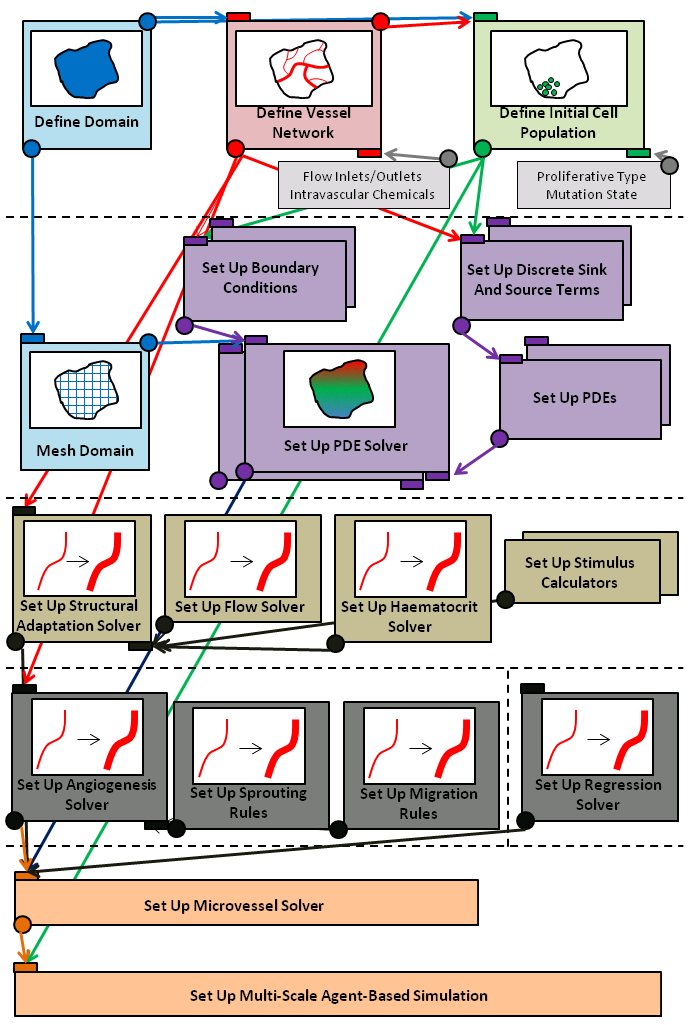
\includegraphics[width=0.9\textwidth]{Fig1.png}
\caption{{\bf An example of how a microvessel model can be composed using Microvessel Chaste.}
A schematic showing the composition of a vascular tumour growth model using Microvessel Chaste. The ability to compose a model from a collection of sub-models and sub-sub-models is noted.}
\label{fig1}
\end{figure}

Fig~\ref{fig2} shows how the library can be used to \emph{solve} a problem of interest in vascular tumour modelling. Again, it is emphasised that the user need not follow the shown solution ordering, but can decide on ordering themselves by suitably over-riding \textit{Solve()} and \textit{Increment()} methods. The steps on the left-hand side of Fig~\ref{fig2} are already implemented as part of the agent-based cell modelling in Chaste~\cite{Mirams2013}. The Microvessel Chaste library interacts with the cell based solver as a plug-in (called a \textit{SimulationModifier} in Chaste), by modifying the contents of a cell population once per time step. In the example problem shown in Fig~\ref{fig2} vessels interact with (non-vessel) cells only via their shared influence on the solutions of chemical transport problems. Cell birth, death and cell-cycle progression can be affected by the PDE solution, which is sampled by each cell during the \textit{CellDataUpdate} step. More detailed interactions, such as cell-vessel spatial occlusion, or forming vessels from collections of discrete cells, are also possible.

\begin{figure}[!h]
\centering
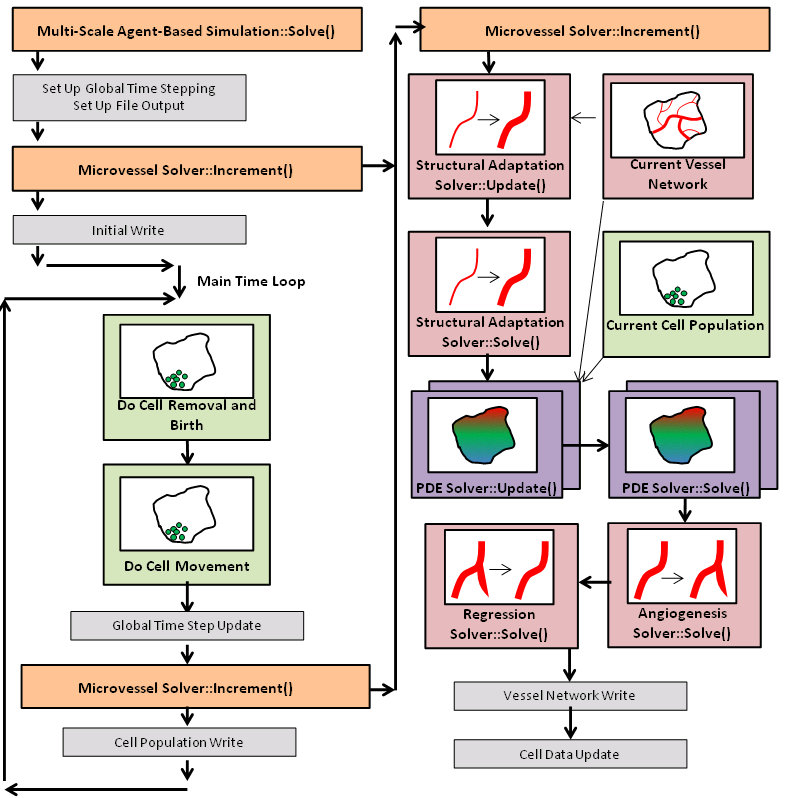
\includegraphics[width=0.8\textwidth]{Fig2.png}
\caption{{\bf An example of how a microvessel model can be solved using Microvessel Chaste.}
A schematic showing the solution of a vascular tumour growth model using Microvessel Chaste. It is noted that solution ordering can be readily changed by the user.}
\label{fig2}
\end{figure}

\subsection*{Code Layout And Design}

The components of the library are as follows:

\begin{itemize}
	\item geometry -- code for generating and describing 2D and 3D geometries using piecewise linear complex (PLC) descriptions for direct use in Triangle [JG add ref] and Tetgen [JG add ref] meshing software,
	\item mesh -- code for automated finite element meshing of 2D and 3D geometries and interpolation of vessel and cell locations onto meshes and regular grids,
	\item ode -- ode models for cell-cycling in vascular tumour problems,
	\item pde -- descriptions and solvers for steady state linear and non-linear PDEs with discrete sinks and sources for vessels and cells. Solvers use finite differences, finite element methods and Green's function methods~\cite{Secomb2013} based on Boost uBLAS and PETSc for vector and matrix operations.
	\item population -- Code for describing, reading, writing and generating vessel networks,
	\item simulation -- flow, structural adaptation and angiogenesis solvers. Also code for managing integration of discrete vessel simulations with discrete cell populations from Chaste.
	\item utility -- Dimensional analysis and collection of literature parameters of interest for tissue microvascualture simulations.	
\end{itemize}

As per the remainder of Chaste, object-oriented programming, including templating in C++ are heavily utilized. Input and output of vessel networks, grids and PDE results are in VTK (Paraview) format, which allows use of standard tools for visualization and post-processing. Python bindings are generated automatically using Py++ with a CASTXML back-end. Pre-compiled C++ classes can be overloaded in Python, without the need to re-compile the full framework. This allows for automated, dynamic model (or sub-model) generation, for example based on the contents of a mark-up language based input file. Given the variety of modelling paradigms and large number of input parameters used in problems of interest, there is much potential for misuse of units. Microvessel Chaste uses low-cost compile-time unit checking to ensure dimensional consistency and automatic solver-specific non-dimensionalisation through the Boost Units framework. The latter is useful for minimising floating pointer errors during the solution of PDEs and flow problems.

\section*{Results}

In this section two sample multi-scale agent-based problems are demonstrated, and are available for reproduction following wiki-based tutorials at \url{https://chaste.cs.ox.ac.uk/trac/wiki/PaperTutorials/Microvessel}.

\subsection*{A 2D Lattice-Based Vascular Tumour Simulation}

The first example is a 2D lattice-based vascular tumour growth simulation following from Owen et al.~\cite{Owen2011}, but with some simplifications to reduce computational expense. This example demonstrates the feasibility of replicating a well known vascular tumour growth simulation, which typifies many others in the literature (JG: add some model refs). It also demonstrates how the library interfaces with the functionality of the Chaste discrete cell modelling software.

The problem is initialized with two large, parallel, counter-flowing vessels, positioned on a regular lattice. A cellular automaton based cell population is used to fill all lattice sites, with `cancer' cell types assigned to a central circular region and `normal' types to the remainder, as shown in Fig~\ref{fig3}. Due to their distance from the large vessels, the tumour cells will become hypoxic and release growth factor (VEGF). This stimulates the growth of new vessels, which migrate preferentially towards the tumour due to growth factor gradients. As shown in Fig~\ref{fig3}, the sprouts can merge if they meet. Vessel diameters can change over time due to blood flow induced stimuli, with vessels with low flow rates eventually removed. New vessels allow for increased oxygenation of the tissue and eventual tumour growth at the expense of immediately surrounding `normal' cells.

There are many potential additions to models of this type which have been explored in the literature, including chemo-therapeutic and anti-angiogeneic drugs[], radiotherapy[] and use of 3D domains[].

% Place figure captions after the first paragraph in which they are cited.
\begin{figure}[!h]
\centering
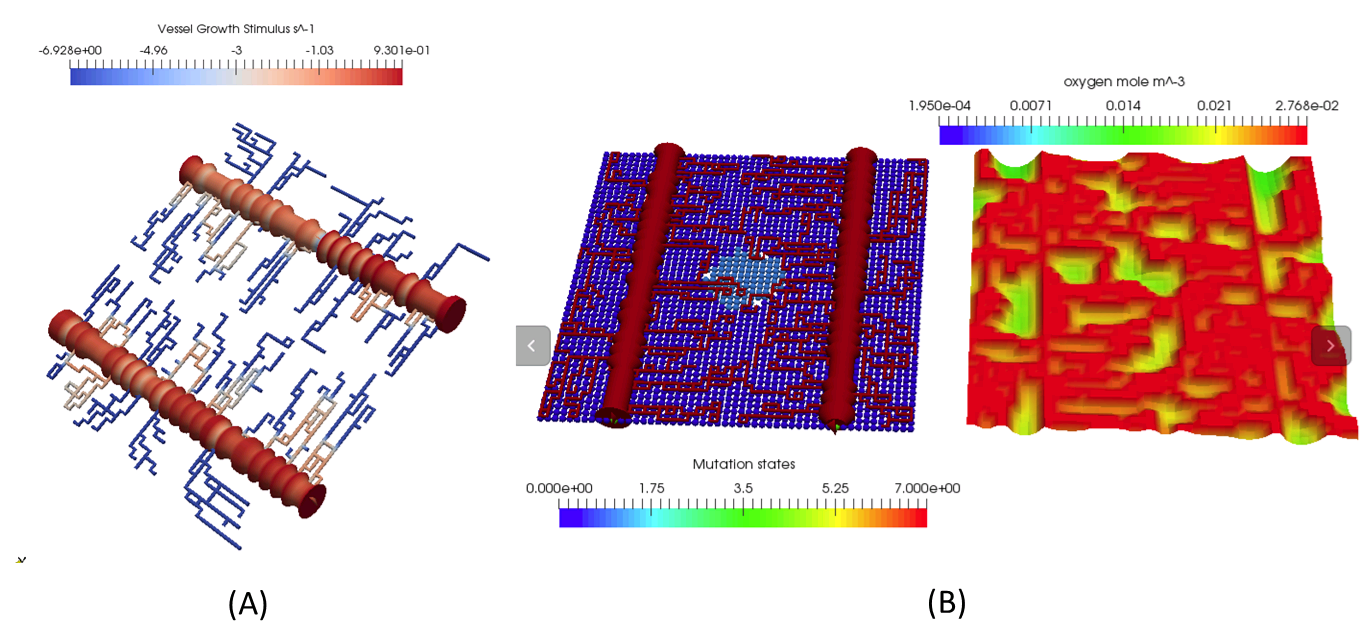
\includegraphics[width=0.99\textwidth]{Fig3.png}
\caption{{\bf A 2D lattice-based vascular tumour simulation performed using the Microvessel Chaste library.}
(A) Top is a sample in-vivo image of tumour cells (green) surrounded by tumour promoted microvascaulture (red), obtained by multi-photon imaging. Bottom is a computational model of a similar vascular tumour growth scenario showing discrete vessels, cells labelled by mutation state and a corresponding oxygen map. (B) A snapshot of the predicted vessel growth stimulus field in response to blood flow. [JG: Scale bars, re-color bottom right to match experimental image. Maybe more specific that not actually modelling the experiment here.]}
\label{fig3}
\end{figure}

\subsection*{A 3D Off-Lattice Angiogenesis Simulation}

The second example is a 3D off-lattice simulation of angiogenesis on a curved surface, shown in Fig~\ref{fig4}. This example demonstrates more advanced features of the library in terms of geometry manipulation, 3D off-lattice angiogenesis and the solution of PDEs on arbitary 3D domains. The application is in modelling the widely used corneal micropocket assay in the study of angiogenesis~\cite{Connor2015}. In this assay a pellet containing a vessel growth stimulus (for example, VEGF) is implanted in the cornea. New vessels sprout from an existing limbal vessel at the base of the cornea and migrate toward the pellet along VEGF gradients. In the computational model discrete cells are excluded. This reduces computational expense for the purposes of generating a tutorial, and corresponds to a widely used modelling paradigm in which cells are treated as a continuum but vessels are modelled discretely~\cite{Secomb2013}. Extensions to this simple model include addition of discrete cells, and multiple vessel growth factors, as per the 2D model in Connor~\emph{et al.}~\cite{Connor2015}.

% Place figure captions after the first paragraph in which they are cited.
\begin{figure}[!h]
\centering
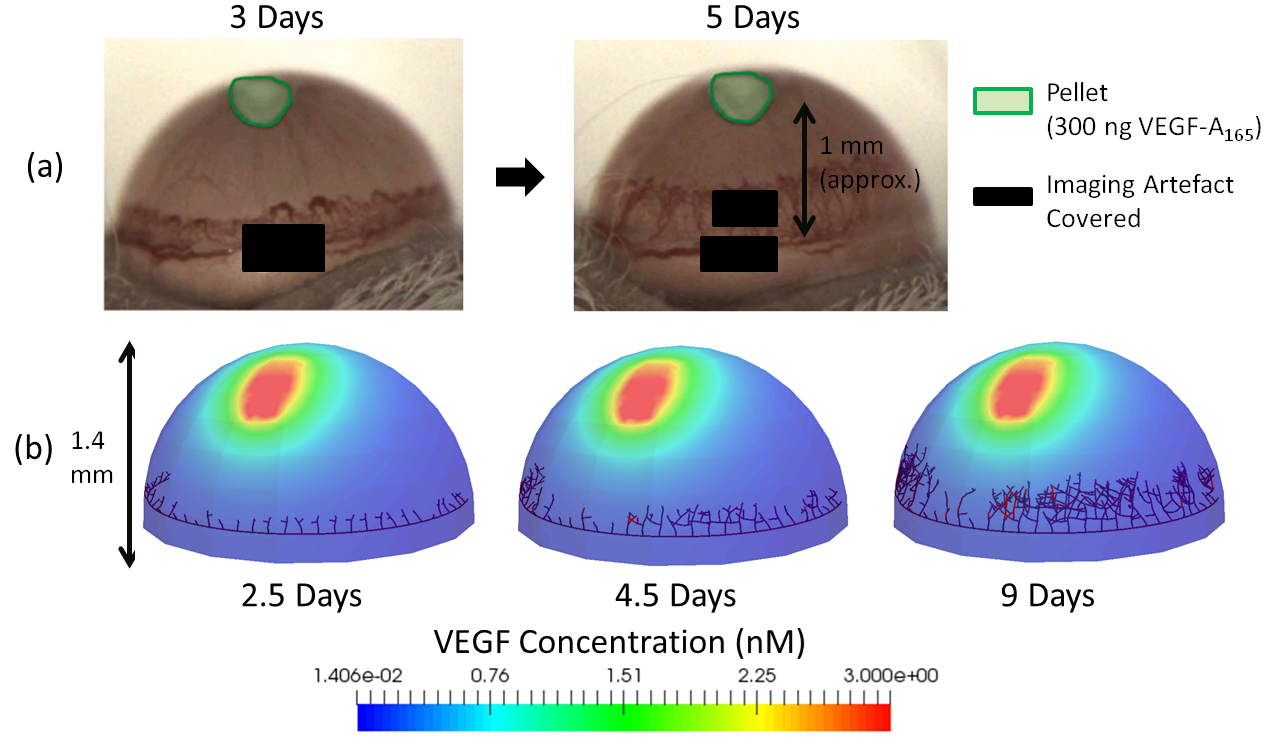
\includegraphics[width=0.99\textwidth]{Fig4.png}
\caption{{\bf A 3D off-lattice angiogenesis simulation performed using the Microvessel Chaste library.}
(A) An example of a corneal micropocket assay highlighting the pellet (green) and growing microvessels (dark red). (B) A corresponding computational simulation showing a predicted VEGF concentration field (nM) and growth of new vessels towards the pellet. [JG add scale bars, fill top right gap with another figure?]}
\label{fig4}
\end{figure}

\section*{Availability and Future Directions}

Microvessel Chaste is available to download from \url{https://chaste.cs.ox.ac.uk/trac/wiki/PaperTutorials/Microvessel} under an open source Berkeley Software Distribution (BSD) licence. Additional functionality for semi-automated 2D and 3D image segmentation and meshing is under development, to aid integration with experimental studies. Porting to Windows and Mac OS X are of interest, with future availability of Python packages for each likely. At present, algorithms operate in serial only, however there is scope for distributed memory parallelisation for both C++ and Python interfaces. All PDE and flow solvers are based on PETSc [] structures and vessel network components may be communicated using existing serialization functionality in Chaste~\cite{Harvey} or through VTK based serialization.

\subsection*{How to Become an Active Developer}

As discussed in Mirams et al.~\cite{Mirams2013}, contributions are welcome via the main Chaste website, which includes a developer wiki, mailing list details and the ability to open and comment on work tickets. 

\section*{Acknowledgments}

[JG Add acknowledgements and funding. Chaste team. Need to ask Bostjan for image permission, then acknowledge. Discuss image permissions with AJ.]

\nolinenumbers

\begin{thebibliography}{10}

\bibitem{Mirams2013}
Mirams GR, Arthurs CJ, Bernabeu MO, Bordas R, Cooper J, Corrias A, Davit Y, Dunn S, Fletcher AG, Harvey DG, Marsh ME, Osborne JM, Pathmanathan P, Pitt-Francis J, Southern J, Zemzemi N, Gavaghan DJ.
\newblock {{C}haste: an open source C++ library for computational physiology and biology}.
\newblock PLoS Comp Bio. 2013 Jan;9(3):e1002970.

\bibitem{Cooper2015}
Cooper J, Spiteri RJ, Mirams GR.
\newblock {{C}ellular cardiac electrophysiology modeling with Chaste and CellML}.
\newblock Front Physiol. 2015 Jan;5:511.

\bibitem{Tetley2016}
Tetley RJ, Blanchard GB, Fletcher AG, Adams RJ, Sanson B.
\newblock {{U}nipolar distributions of junctional Myosin II identify cell stripe boundaries that drive cell intercalation throughout Drosophila axis extension}.
\newblock eLife. 2016 May;5:e12094.

\bibitem{Dunn2016}
Dunn SJ, Osborne JM, Appleton PL, Nathke I.
\newblock {{C}ombined changes in Wnt signaling response and contact inhibition induce altered proliferation in radiation-treated intestinal crypts}.
\newblock Mol Biol Cell. 2016 June;27(11):1863-1874.

\bibitem{Figueredo2013}
Figueredo GP, Joshi TV, Osborne J, Byrne HM, Owen MR.
\newblock {{O}n-lattice agent-based simulation of populations of cells within the open-source Chaste framework}.
\newblock Interface Focus. 2013 February;3(2):e20120081.

\bibitem{Owen2011}
Owen MR, Stamper J, Muthana M, Richardshon GW, Dobson J, Lewis CE, Byrne HM.
\newblock {{M}athematical modeling predicts synergistic antitumor effects of combining a macrophage-based, hypoxia-targeted gene therapy with chemotherapy}.
\newblock Cancer Res. 2015 April;71(8):2826-2837.

\bibitem{Swat2012}
Swat M, Thomas GL, Belmonte JM, Shirinifard A, Hmeljak D, Glazier JA.
\newblock {{M}ulti-scale modeling of tissues using CompuCell3D}.
\newblock Method in Cell Biol. 2012;110:325-366.

\bibitem{Sutterlin2013}
Sutterlin T, Kolb C, Dickhaus H, Jager D, Grabe N.
\newblock {{B}ridging the scales: semantic integration of quantitative SBML in graphical multi-cellular models and simulations with EPISIM and COPASI}.
\newblock Bioinformations. 2013 January;15(29):223-229.

\bibitem{Macklin2012}
Macklin P, Edgerton ME, Thompson AM, Cristini V.
\newblock {{P}atient-calibrated agent-based modelling of ductal carcinoma in situ (DCIS): From microscopic measurements to macroscopic predictions of clinical progression}.
\newblock J Theor Biol. 2012;301:122-140.

\bibitem{boost161}
Boost Development Team.
\newblock {{B}oost Units Reference Guide}.
\newblock Available: \url{http://www.boost.org/doc/libs/1_61_0/doc/html/boost_units.html}.

\bibitem{Secomb2013}
Secomb TW, Alberding JP, Hsu R, DeWhirst MW, Pries AR.
\newblock {{A}ngiogenesis: an adaptive dynamic biological patterning problem}.
\newblock PLoS Comp Bio. 2013;9(3):e1002983.

\bibitem{Anderson1998}
Anderson ARA, Chaplain MAJ.
\newblock {{C}ontinuous and discrete mathematical models of tumor-induced angiogenesis}.
\newblock Bullet Math Bio. 1998;60:857-900.

\bibitem{Frieboes2007}
Frieboes HB, Lowengrub JS, Wise S, Zheng X, Macklin P, Bearer E, Cristini V.
\newblock {{C}omputer simulation of glioma growth and morphology}.
\newblock Neuroimage. 2007;37(Supl 1):S59-S70.

\bibitem{Shirinifard2009}
Shirinifard A, Scott Gens J, Zaitlen L, Poplawski J, Swat M, Glazier JA.
\newblock {{3}D multi-cell simulation of tumor growth and angiogenesis}.
\newblock PLoS One. 2009;4(10):e7190.

\bibitem{Welter2013}
Welter M, Rieger H.
\newblock {{I}nterstitial fluid flow and drug delivery in vascularized tumors: a computational model}.
\newblock PLoS One. 2013;8(8):e70395.

\bibitem{Alarcon2005}
Alarcon T, Byrne HM, Maini PK.
\newblock {{A} multiple scale model for tumor growth}.
\newblock Multiscale model simul. 2005;3(2):440-475.

\bibitem{Perfahl2011}
Perfahl H, Byrne HM, Chen T, Estrella V, Alarcon T, Lapin A, Gatenby R, Gillies RJ, Llord MC, Maini PK, Reuss M, Owen MR.
\newblock {{M}ultiscale modelling of vascular tumour growth in 3D: the roles of domain size and boundary conditions}.
\newblock PLoS One. 2011 April;6(4):e14790.

\bibitem{Connor2015}
Connor AJ, Radoslaw P, Nowak EL, Thomas M, Hertig F, Hoert S, Quaiser T, Schocat E, Pitt-Francis J, Cooper J, Maini PK, Byrne HM.
\newblock {{A}n integrated approach to quantitative modelling in angiogenesis research}.
\newblock J R Soc Interface. 2015 August;12:e20150546.

\bibitem{Rieger2015}
Rieger H, Welter M.
\newblock {{I}ntegrative models of vascular remodeling during tumor growth}.
\newblock WIREs Syst Biol Med. 2015;7:113-129.

\bibitem{Connor2012}
Connor AJ, Cooper J, Byrne HM, Maini PK, McKeever S.
\newblock {{O}bject-oriented paradigms for modelling vascular tumor growth: a case study}.
\newblock In: The Fourth International Conference on Advances in Systems Simulation. Simul 2012. Iaria, Lisbon,74-83.

\bibitem{Tozer2004}
Tozer GM, Ameer-Berg SM, Baker J, Barber P, Hill SA, Hodgkiss R, Locke R, Prise V, Wilson I, Vojnovic B.
\newblock {{I}ntravital imaging of tumour vascular networks using multi-photon fluorescence microscopy}.
\newblock Advanced Drug Deliv Rev. 2005;57:135-152.

\bibitem{Grogan2016}
Grogan JA, Markelc B, Connor AJ, Muschel R, Pitt-Francis JM, Maini PK, Byrne HM.
\newblock {{P}redicting the influence of microvascular structure on tumour response to radiotherapy}.
\newblock IEEE Trans Biomed Eng 2016;In Press,DOI:10.1109/TBME.2016.2606563.

\bibitem{bib2}
Ohno S.
\newblock Evolution by gene duplication.
\newblock London: George Alien \& Unwin Ltd. Berlin, Heidelberg and New York:
  Springer-Verlag.; 1970.

\bibitem{bib3}
Magwire MM, Bayer F, Webster CL, Cao C, Jiggins FM.
\newblock {{S}uccessive increases in the resistance of {D}rosophila to viral
  infection through a transposon insertion followed by a {D}uplication}.
\newblock PLoS Genet. 2011 Oct;7(10):e1002337.

\end{thebibliography}



\end{document}

